
% ===========================
\chapter{Konzept}
\label{konzept}
% ===========================

Wie in Abschnitt \ref{grundlagen_fahren} beschrieben, stellt das Testen von hochautomatisierten \ac{FAS} die Automobilindustrie vor große Herausforderungen. Die Menge der bekannten Fahrszenarien ist nur eine Teilmenge aller Szenarien, die zukünftige \ac{FAS} abdecken müssen. Diese Beziehung ist schematisch in Abbildung \ref{fig_teilmenge_fahrszenarien} dargestellt. Die Folge ist eine steigende Anzahl benötigter Testkilometer, die in Zukunft mit ökonomischem Aufwand nicht mehr umsetzbar sein wird. Es müssen neue Methoden gefunden werden, relevante Szenarien für die Generierung von Testfällen zu identifizieren, um die Sicherung von hochautomatisierten \ac{FAS} mit ökonomischen Aufwand garantieren zu können.

Genau hier soll diese Arbeit einen Beitrag leisten. Das Ziel, wie bereits in Abschnitt \ref{einleitung_zielsetzung} erläutert, ist die Identifikation von bisher unbekannten Fahrszenarien. Die Grundidee ist es einen Klassifikator mit einem großen Anteil synthetischer Daten und einem kleinen Anteil realer Daten von bisher bekannten Szenarien zu trainieren. Dieser Klassifikator kann dann bekannte Szenarien erkennen, liefert aber keine eindeutigen Ergebnisse bei bisher unbekannten Szenarien. Mit dieser Methodik soll es möglich sein bisher unbekannte Fahrszenarien zu identifizieren, um auf der Basis neue Testfälle für die Sicherung hochautomatisierter Fahrfunktionen zu generieren.

\begin{figure}[h]
\centering
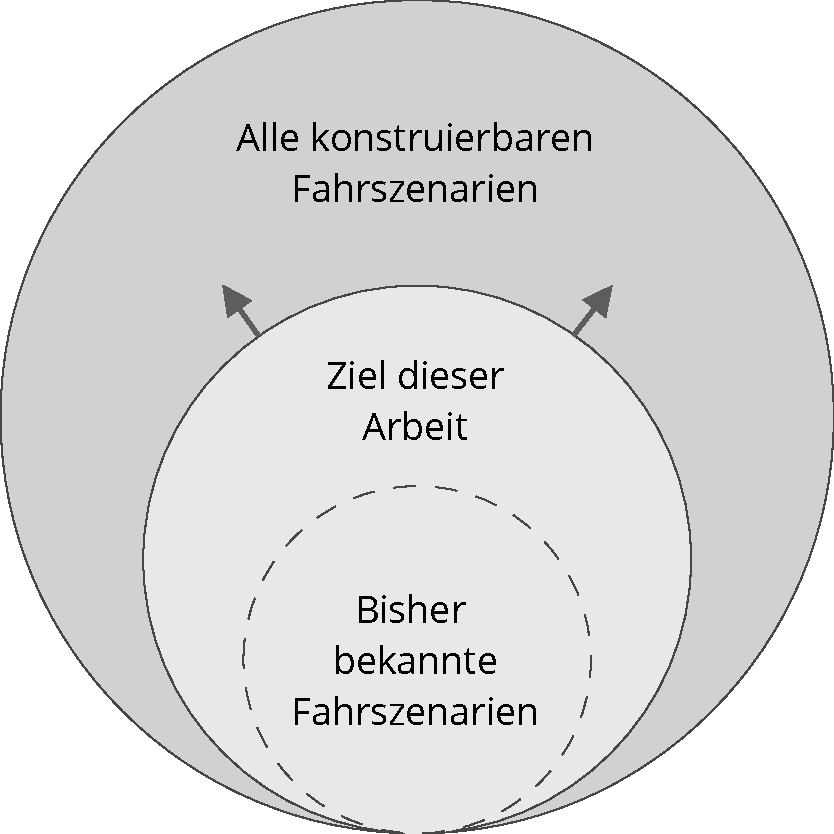
\includegraphics[scale=0.3]{teilmenge_fahrszenarien.pdf}
\caption{Beziehung zwischen bekannten und unbekannten Fahrszenarien}
\label{fig_teilmenge_fahrszenarien}
\end{figure}

In dieser Arbeit soll ein Proof-of-Concept für diese Methodik entwickelt werden. Dafür wird im folgenden Abschnitt \ref{konzept_struktur} das Konzept im Detail und die Vorgehensweise vorgestellt. Anschließend wird in Abschnitt \ref{konzept_methodik} die Methodik erklärt mit welcher dieses Konzept umgesetzt werden soll.


% ===========================
\section{Struktur}
\label{konzept_struktur}
% ===========================

Die Umsetzung in dieser Arbeit lässt sich in drei Teile untergliedern. Im ersten Teil werden die zu klassifizierenden Szenarien als \textit{logische Szenarien} definiert. Auf der Basis werden im zweiten Teil synthetische und reale Trainingsdaten generiert. Im dritten Teil wird schließlich ein \ac{KNN} als Klassifikator trainiert und evaluiert. Diese Struktur ist schematisch in Abbildung \ref{fig_konzept_struktur} abgebildet und wird in den folgenden Absätzen weiter beschrieben.

\begin{figure}[h]
\centering
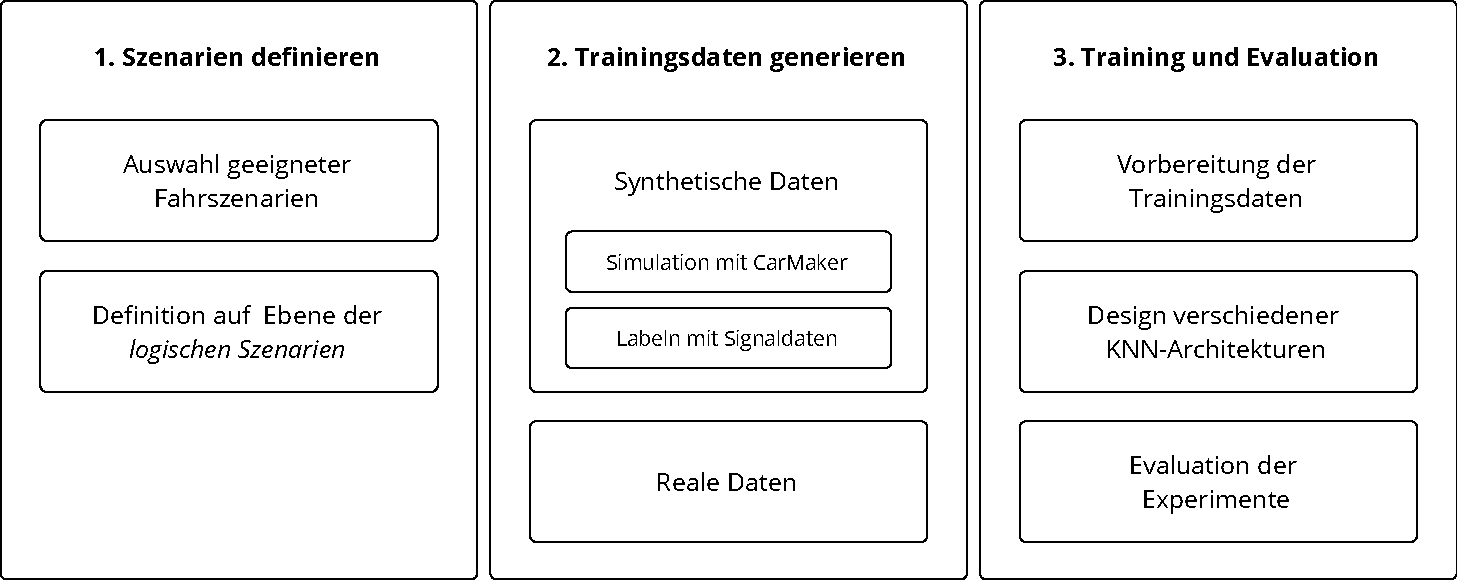
\includegraphics[scale=0.6]{konzept_struktur.pdf}
\caption{Konzept dieser Arbeit}
\label{fig_konzept_struktur}
\end{figure}

Im ersten Schritt der Umsetzung werden bestimmte Fahrszenarien ausgewählt und wie in Abschnitt \ref{grundlagen_fahren_szenarien} definiert. In dieser Arbeit werden Szenarien auf der Ebene der \textit{logischen Szenarien} definiert. Nachdem Szenarien ausgewählt und definiert sind, werden synthetische und reale Daten für das Training eines Klassifikators benötigt.

Für die Generierung von synthetischen Daten wird mit der Simulationssoftware CarMaker gearbeitet. Mit dieser Software können das Ego-Fahrzeug, Straßen, Verkehr und die Trajektorien aller Fahrzeuge generiert und beliebig verändert werden. Die Idee ist es, Fahrten des Ego-Fahrzeugs zu simulieren, entsprechende Bild- und Signaldaten aufzuzeichnen und die Bilddaten anhand der Signaldaten zu labeln. Auf diese Weise können ohne großen Aufwand beliebig viele synthetische Daten erzeugt und gelabelt werden. Mit CarMaker können sowohl Rohdaten, wie zum Beispiel Radarsignale des Ego-Fahrzeugs, als auch abstrakte Informationen, wie die Position und Geschwindigkeit von anderen Objekten, simuliert werden. Amersbach und Winner \cite{amersbach2017functional} stellen einen Ansatz für die funktionale Dekomposition von hochautomatisierten \ac{FAS} vor. In diesem Ansatz werden Informationen über sechs Schichten, von den Ground Truth Daten über die Szenenerkennung bis zur entsprechenden Aktion des Ego-Fahrzeugs, abgeleitet. Ein Schema dieses Ansatzes ist in Abbildung \ref{fig_functional_decomposition} dargestellt. In dieser Arbeit werden für das Labeln der Bilddaten Signaldaten generiert, die nach Schicht 1 (e.g. Geschwindigkeit des Ego-Fahrzeugs) und Schicht 2 (e.g Position des vorausfahrenden Fahrzeugs) eingeordnet werden können. Jeder generierte Zeitpunkt stellt eine Szene, wie in Abschnitt \ref{grundlagen_fahren_szenarien} beschrieben, dar. Jede Szene wird separat auf Basis der entsprechenden Signaldaten nach festgelegten Regeln klassifiziert. Die Aneinanderreihung von mehreren Szenen ergibt schließlich ein Szenario. Für die Generierung von realen Trainingsdaten werden Videosequenzen verwendet und manuell gelabelt.

\begin{figure}[h]
\centering
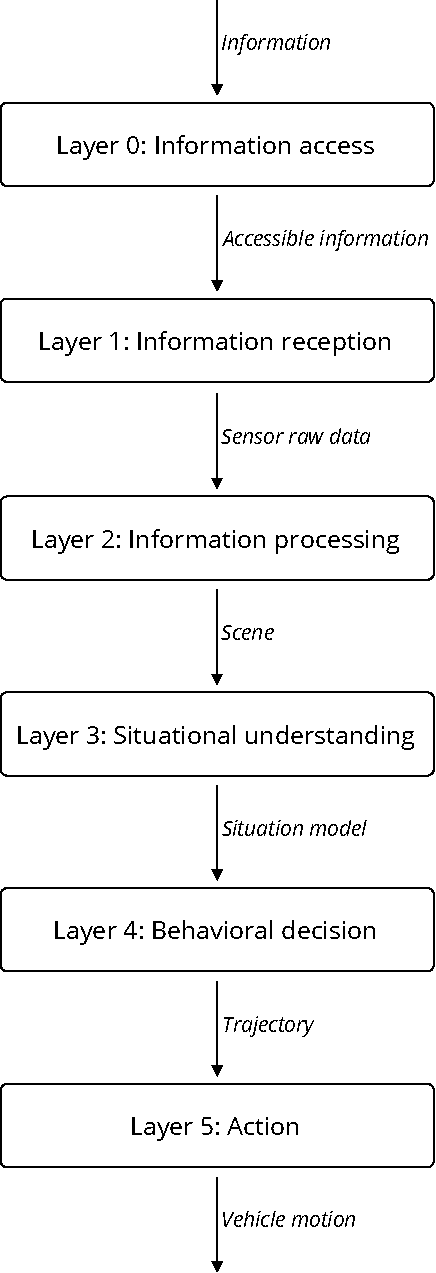
\includegraphics[scale=0.5]{functional_decomposition.pdf}
\caption{Schema der funktionalen Dekomposition \cite{amersbach2017functional}}
\label{fig_functional_decomposition}
\end{figure}

Für das Training und die Evaluation eines Klassifikators werden \acp{KNN} verwendet. Wie in Abschnitt \ref{grundlagen_nn} beschrieben, sind \acp{CNN} nach dem Stand der Technik die besten Architekturen um Merkmale aus Bildern zu extrahieren. \acp{LSTM} sind besonders für Zeitreihen geeignet. Daher wird ein Klassifikator aus einer Kombination dieser Architekturen erstellt. Um die Skalierbarkeit dieses Ansatzes zu gewährleisten, wird für das Training nur ein kleiner Teil realer und ein großer Teil synthetischer Daten verwendet. Damit wird auch für die Zukunft der Aufwand des manuellen Labelns gering gehalten.


% ===========================
\section{Ansätze, Methoden, Werkzeuge}
\label{konzept_methodik}
% ===========================

In diesem Abschnitt wird ein Überblick gegeben, welche Ansätze, Methoden und Werkzeuge in den jeweiligen Teilen der Umsetzung verwendet werden. Diese Zuordnung ist in der folgenden Tabelle \ref{tab_konzept_methods} dargestellt. Die detaillierte Beschreibung folgt in Kapitel \ref{umsetzung}.

\small
\begin{longtable}[c]{p{5cm} p{6.5cm} p{1.5cm}}
\textbf{Teil der Umsetzung} & \textbf{Ansätze, Methoden, Werkzeuge} & \textbf{Quellen} \\
\hline
\endhead

Auswahl und Definition geeigneter Fahrszenarien & Konzept der \textit{logischen Szenarien} & \cite{ulbrich2015defining}, \cite{bagschik2017szenarien} \\
\hline
Simulation und Labeln synthetischer Trainingsdaten & Generierung von Bild- und Signaldaten mit CarMaker, regelbasierte Klassifizierung auf Basis von vorher festgelegten Signaldaten & Gegenstand dieser Arbeit \\
\hline
Generierung realer Trainingsdaten & Auswahl geeigneter Videosequenzen von YouTube, manuelles Labeln & Gegenstand dieser Arbeit \\
\hline
Vorbereitung der Daten, Erstellung des Klassifikators und Evaluation der Experimente & Architektur eines \ac{KNN} mit einer Kombination von \ac{CNN} und \ac{LSTM}, implementiert mit Python und Keras & \cite{chollet2015keras}, CNN, LSTM \\

\hline
\caption{Ansätze, Methoden und Werkzeuge dieser Arbeit}
\label{tab_konzept_methods}
\end{longtable}
\normalsize




